\documentclass[a4paper,12pt]{article} % This defines the style of your paper

\usepackage[top = 2.5cm, bottom = 2.5cm, left = 2.5cm, right = 2.5cm]{geometry} 
\usepackage[utf8]{inputenc} %utf8 % lettere accentate da tastiera
\usepackage[english]{babel} % lingua del documento
\usepackage[T1]{fontenc} % codifica dei font

\usepackage{multirow} % Multirow is for tables with multiple rows within one 
%cell.
\usepackage{booktabs} % For even nicer tables.

\usepackage{graphicx} 

\usepackage{setspace}
\setlength{\parindent}{0in}

\usepackage{float}

\usepackage{fancyhdr}

\usepackage{caption}
\usepackage{amssymb}
\usepackage{amsmath}
\usepackage{mathtools}
\usepackage{color}

\usepackage[hidelinks]{hyperref}
\usepackage{csquotes}
\usepackage{subfigure}

\usepackage{ifxetex,ifluatex}
\usepackage{etoolbox}
\usepackage[svgnames]{xcolor}

\usepackage{tikz}

\usepackage{framed}

 \newcommand*\quotefont{\fontfamily{LinuxLibertineT-LF}} % selects Libertine as 
 %the quote font


\newcommand*\quotesize{40} % if quote size changes, need a way to make shifts 
%relative
% Make commands for the quotes
\newcommand*{\openquote}
{\tikz[remember picture,overlay,xshift=-4ex,yshift=-1ex]
	\node (OQ) 
	{\quotefont\fontsize{\quotesize}{\quotesize}\selectfont``};\kern0pt}

\newcommand*{\closequote}[1]
{\tikz[remember picture,overlay,xshift=4ex,yshift=-1ex]
	\node (CQ) {\quotefont\fontsize{\quotesize}{\quotesize}\selectfont''};}

% select a colour for the shading
\colorlet{shadecolor}{WhiteSmoke}

\newcommand*\shadedauthorformat{\emph} % define format for the author argument

% Now a command to allow left, right and centre alignment of the author
\newcommand*\authoralign[1]{%
	\if#1l
	\def\authorfill{}\def\quotefill{\hfill}
	\else
	\if#1r
	\def\authorfill{\hfill}\def\quotefill{}
	\else
	\if#1c
	\gdef\authorfill{\hfill}\def\quotefill{\hfill}
	\else\typeout{Invalid option}
	\fi
	\fi
	\fi}
% wrap everything in its own environment which takes one argument (author) and 
%one optional argument
% specifying the alignment [l, r or c]
%
\newenvironment{shadequote}[2][l]%
{\authoralign{#1}
	\ifblank{#2}
	{\def\shadequoteauthor{}\def\yshift{-2ex}\def\quotefill{\hfill}}
	{\def\shadequoteauthor{\par\authorfill\shadedauthorformat{#2}}\def\yshift{2ex}}
	\begin{snugshade}\begin{quote}\openquote}
		{\shadequoteauthor\quotefill\closequote{\yshift}\end{quote}\end{snugshade}}

\newcommand{\footref}[1]{%
	$^{\ref{#1}}$%
}

\pagestyle{fancy}

\setlength\parindent{24pt}

\fancyhf{}

\lhead{\footnotesize Deep Learning Lab: Assignment 3}

\rhead{\footnotesize Giorgia Adorni}

\cfoot{\footnotesize \thepage} 

\begin{document}
	\thispagestyle{empty}  
	\noindent{
	\begin{tabular}{p{15cm}} 
		{\large \bf Deep Learning Lab} \\
		Università della Svizzera Italiana \\ Faculty of Informatics \\ \today  \\
		\hline
		\\
	\end{tabular} 
	
	\vspace*{0.3cm} 
	
	\begin{center}
		{\Large \bf Assignment 3: Long Short-Term Memory Network}
		\vspace{2mm}
		
		{\bf Giorgia Adorni (giorgia.adorni@usi.ch)}
		
	\end{center}  
}
	\vspace{0.4cm}

	%%%%%%%%%%%%%%%%%%%%%%%%%%%%%%%%%%%%%%%%%%%%%%%%
	%%%%%%%%%%%%%%%%%%%%%%%%%%%%%%%%%%%%%%%%%%%%%%%%
	
	\section{Introduction}
	\label{section:intro}
	The goal of this project is to implement a text generator based on Long 
	Short-Term Memory (LSTM).
	
	\section{Preprocessing}
	\label{section:preprocessing}
	First of all, the book \textit{The Count of Monte Cristo} has been  
	downloaded in plain English text from Project Gutenberg.
	
	The first operation performed consists in the conversion to lower case of 
	all the text characters. Afterwards, a simple analysis of the data was 
	performed.
	
	The book contains about 2.65 million characters and in total there are 
	$111$ unique characters. The character list is displayed in Figure 
	\ref{fig:initial}, and it can be seen that the book contains English 
	letters, number, punctuation, symbols and Greek letters.
	
	\begin{figure}[htb]
		\centering
		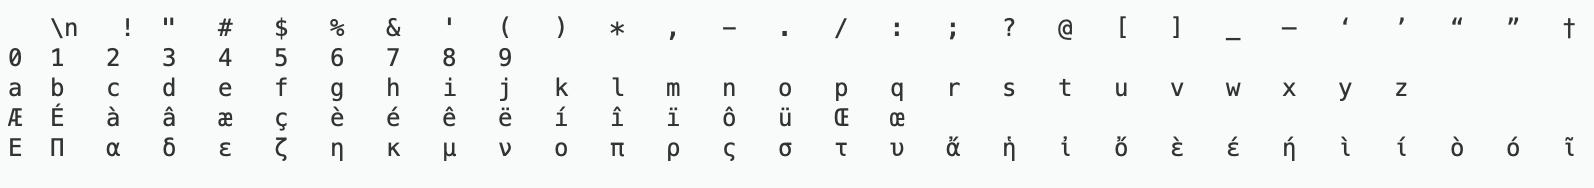
\includegraphics[width=\linewidth]{initial.png}	
		\caption{Unique characters in \textit{The Count of Monte Cristo}}
		\label{fig:initial}
	\end{figure}

 	In order to train the network, it is necessary to map the text strings to a 
 	numerical representation. First of all,	the number of unique characters 
 	were counted as well as the absolute and relative frequencies. Hence, two 
 	dictionaries that act as lookup tables are created: one mapping characters 
 	to integers, and the other integers to characters. This will be crucial for 
 	the creation of a one-hot encoding.
 	
 	In Table \ref{tab:statistics} are presented the $20$ most frequent 
 	characters, with the corresponding encodings and frequencies.
	
	\begin{figure}[htb]
		\centering
		\begin{tabular}{llcc}
			\toprule
			Encoding & Characters &  Absolute Frequencies & Relative 
			Frequencies \\
			\midrule
			8        &           &              420940 &            15.901\% \\
			5        &         e &              259094 &             9.787\% \\
			7        &         t &              180542 &              6.82\% \\
			21       &         a &              165546 &             6.253\% \\
			3        &         o &              157076 &             5.933\% \\
			18       &         i &              142302 &             5.375\% \\
			11       &         n &              137584 &             5.197\% \\
			14       &         s &              126590 &             4.782\% \\
			15       &         h &              126368 &             4.773\% \\
			2        &         r &              121407 &             4.586\% \\
			24       &         d &               94099 &             3.554\% \\
			22       &         l &               80730 &             3.049\% \\
			0        &        \textbackslash n &               61739 
			& 2.332\% \\
			10       &         u &               60318 &             2.278\% \\
			17       &         m &               57157 &             2.159\% \\
			6        &         c &               52526 &             1.984\% \\
			16       &         f &               45383 &             1.714\% \\
			19       &         , &               45246 &             1.709\% \\
			27       &         w &               43892 &             1.658\% \\
			20       &         y &               42642 &             1.611\% \\
			\dots       &         \dots &                \dots &             
			\dots 
			\\
			\bottomrule
		\end{tabular}
		\captionof{table}{Encoding and frequencies of the most frequent 
		characters}
		\label{tab:statistics}
	\end{figure}

	\bigskip
	Soon after, training examples and targets were created. The input examples 
	correspond to a sequence of characters, while the target of each character 
	corresponds to the following character in the original sequence. In this 
	way, there is no target for the last element of the sequence.
	
	\section{Truncated backpropagation through time}
	\label{section:backpropagation}
	
	Given a very long sequence, it is impossible to feed it entirely and 
	then compute the backpropagation. Instead, it is possible to divide the 
	sequence into $n$ blocks and each block in $m$ subsequences which contain a 
	fixed number of characters of the text.\bigskip
	
	The $i\mathrm{-th}$ batch is created taking the $i\mathrm{-th}$ subsequence 
	from each block and computing the backpropagation on it. In this way, each 
	batch has multiple subsequences and the computations are more efficient.
	
	This approach enables us to pass the output state of a batch as input state 
	of the next batch. The state is reset to zero at the beginning of each 
	epoch.\bigskip
	
	In the experiment that will be presented have been used 16 blocks with 
	subsequences of size 256. 
	To ensure that all batches have sequences of the same length, before 
	creating the batches, the text is padded in such a way that sequences that 
	are shorter than 256 are filled with 0 at the end, thus avoiding to 
	truncate them.
	
	A mask containing the index of the valid characters is created in order to 
	compute the loss.
	
	\section{Network}
	\label{section:network}
	
	The model implemented is composed of a MultiRNNCell with two LSTMCells each 
	containing 256 units, following by a softmax output layer with $k$ units, 
	which correspond to the number of unique characters (one-hot encoding), in 
	this case 111.
	
	Table \ref{tab:model0} summarises the architecture of the network used in 
	the first experiment.	
	\begin{figure}[htb]
		\centering
		
		\begin{tabular}{ccc}
			\toprule
			\textbf{LSTMCell1} & \textbf{LSTMCell2} & \textbf{softmax} \\
			\midrule
			256 & 256 & 111\\
			\bottomrule
		\end{tabular}
		\captionof{table}{Network architecture}
		\label{tab:model0}
	\end{figure}

	\section{Evolution of the training loss function}
	\label{section:loss}

	The training would take 5 epochs and Adam is used as optimiser with a 
	learning rate of $10^2$. As loss function, the Softmax Cross Entropy with 
	Logits is used since the problem can be treated as a classification one.
	
	All the models were implemented using TensorFlow and trained on an NVIDIA 
	Tesla V100-PCIE-16GB GPU.
	
	The training loss of this experiment is shown in Figure 
	\ref{fig:model0-loss}.
	
	\begin{figure}[htb]
		\centering
		\includegraphics[width=.7\linewidth]{../src/out/initial/img/loss.pdf}	
		\caption{Training loss}
		\label{fig:model0-loss}
	\end{figure}

	The training loss at the end of the last epoch is 1.32.
	It is clearly visible that the training loss is still decreasing, so in a
	further modification of the model, presented in Section 
	\ref{section:improvement}, will be analysed the possibility of 
	increasing the number of training epochs in order to improve the results.

	\section{Generate and document 20 sequences}
	After training the model, in order to evaluate the network, 20 sequences 
	composed of 256 characters are generated.\bigskip
	
	The procedure of generation of a sequence starts by choosing an initial 
	character randomly, based on the relative frequencies presented in Section 
	\ref{section:preprocessing}.
	
	After that, the prediction distribution of the next character is given 
	using the initial character and the state of the network. In order to 
	calculate the index of the predicted character, a categorical distribution 
	is used. 
	
	The predicted character is used as the following input of the model along 
	with the previous hidden state.\bigskip

	\noindent	Below, the 20 sequences generated are shown:
	\begin{shadequote}{}
		5sat\texttt{$\backslash$n}\\
		promisence, clatood rumbs if he had been belong and the approached 
		my general promises remained for me, not me, really seem you tractly 
		second shoulders.{$\backslash$n}\\
		{$\backslash$n}\\
		“means to your other with them.”{$\backslash$n}\\
		{$\backslash$n}\\
		“do not spoke when the orssused assisting his color{$\backslash$n}\\
		upon{$\backslash$n}\\
		the s
	\end{shadequote}

	\begin{shadequote}{}
		6strel—shall\texttt{$\backslash$n}\\
		remate (to?”\texttt{$\backslash$n}\\
		\texttt{$\backslash$n}\\
		“well,” said the don his deformined to spaftly had 
		mig.”\texttt{$\backslash$n}\\
		\texttt{$\backslash$n}\\
		“wnaties; and he a name; but natuon mine of an enellem masters, making 
		frequently smilings of many time?” she said. this great convinced with
		mucious accutth the dround th
	\end{shadequote}
	
	\begin{shadequote}{}
		t\texttt{$\backslash$n}\\
		dantès was\texttt{$\backslash$n}\\
		in yous hears litenance. “he keyess withsser?”\texttt{$\backslash$n}\\
		\texttt{$\backslash$n}\\
		“well,” returned madame he has valentine was a man, to request from 
		valentine.”\texttt{$\backslash$n}\\
		\texttt{$\backslash$n}\\
		“ah, do you will understand it not makes.\texttt{$\backslash$n}\\
		\texttt{$\backslash$n}\\
		50257m\texttt{$\backslash$n}\\
		\texttt{$\backslash$n}\\
		\texttt{$\backslash$n}\\
		\texttt{$\backslash$n}\\
		“go,” edmond words agried. which five about of the scarce boo
	\end{shadequote}

	\begin{shadequote}{}
		called\texttt{$\backslash$n}\\
		byoustion\texttt{$\backslash$n}\\
		since the old man, “whom best alone than assopeated the corner of 
		the\texttt{$\backslash$n}\\
		continued dansèled that instant themselves milling only constances i 
		will 
		debray has\texttt{$\backslash$n}\\
		been\texttt{$\backslash$n}\\
		albert unlived its at the same worthy table of 
		which\texttt{$\backslash$n}\\
		another through me to ong 
	\end{shadequote}
		
	\begin{shadequote}{}
		slock\texttt{$\backslash$n}\\
		in their it by having appearer whom do not made that had impossible 
		plance 
		the \_whole nighted box. “that he exciteed all wildieu,” 
		replied\texttt{$\backslash$n}\\
		debral presence combriction of the maxitelos in this 
		parison\texttt{$\backslash$n}\\
		and projective was took this deadly storp by at te
	\end{shadequote}
	
	\begin{shadequote}{}
		stillow was creek of our entire?”\texttt{$\backslash$n}\\
		\texttt{$\backslash$n}\\
		“alas? dantès (and crime frécapans he, under their appressions of 
		themselves found and you too goved you about conccarce a
		gendarmes.\texttt{$\backslash$n}\\
		\texttt{$\backslash$n}\\
		“of their cloud that offering emotion?”\texttt{$\backslash$n}\\
		\texttt{$\backslash$n}\\
		“oh, yes; brown of them, like today created 
	\end{shadequote}
	
	\begin{shadequote}{}
		respect of any composed me of cleaked on golden\texttt{$\backslash$n}\\
		out of a word to after his mothed them with\texttt{$\backslash$n}\\
		stidned with and murder of the count shill long memble and my days of 
		announceplies celeased his man, and spazz marsen 
		me.”\texttt{$\backslash$n}\\
		\texttt{$\backslash$n}\\
		“alaply feeling really\texttt{$\backslash$n}\\
		below.”\texttt{$\backslash$n}\\
		\texttt{$\backslash$n}\\
		“and is
	\end{shadequote}
	
	\begin{shadequote}{}
		lemmores a gazed to the\texttt{$\backslash$n}\\
		shadon of brains to m. de villet, that serias,\texttt{$\backslash$n}\\
		spoken to looking one of his from the six fately\texttt{$\backslash$n}\\
		strange to\texttt{$\backslash$n}\\
		seemed there of in-lacquent from\texttt{$\backslash$n}\\
		nothing\texttt{$\backslash$n}\\
		called to atpen what deserved that is his accous, for any placed my 
		partes.”\texttt{$\backslash$n}\\
		\texttt{$\backslash$n}\\
		“undes
	\end{shadequote}
	
	\begin{shadequote}{}
		led and still proof venigality left?”\texttt{$\backslash$n}\\
		\texttt{$\backslash$n}\\
		“have he has from medound, and when an occond 
		detailed.”\texttt{$\backslash$n}\\
		\texttt{$\backslash$n}\\
		“complexcessed two voice corled that just have\texttt{$\backslash$n}\\
		his pater fuxent and odden of gentlemen watched to ut leave 
		heambsimally 
		told me a yestrioled with anotanted att
	\end{shadequote}
	
	\begin{shadequote}{}
		ded i have found understand,\texttt{$\backslash$n}\\
		that to has genessed woodenate stalus which promise to gotn, breaunden 
		one 
		with an exclamatual\texttt{$\backslash$n}\\
		possessed themselve than which not accustomed withspaper as followed me 
		sister, to mensions to place in them converse was followed a
	\end{shadequote}
	
	\begin{shadequote}{}
		exts his words riving a—wailing out, which beligualles had sufficed her 
		conquponor had to consime offering with the count’s diamonds of
		franz; “my officent\texttt{$\backslash$n}\\
		ship to villefort regend\texttt{$\backslash$n}\\
		franz had been sailed a young\texttt{$\backslash$n}\\
		in\texttt{$\backslash$n}\\
		subject which were on boused by a fext to
	\end{shadequote}
	
	\begin{shadequote}{}
		yselve to believe\texttt{$\backslash$n}\\
		me by an\texttt{$\backslash$n}\\
		innocend, “where he befoced over\texttt{$\backslash$n}\\
		only here greeks, which\texttt{$\backslash$n}\\
		always like me make,\texttt{$\backslash$n}\\
		cherusbated 1.1..................6... ladded villefort; “what know on 
		them 
		for assolity to themselves them; you alough the leat or blood and 
		lamber, st
		
	\end{shadequote}
	
	\begin{shadequote}{}
		íbandrally orden-clouds.\texttt{$\backslash$n}\\
		\texttt{$\backslash$n}\\
		the\texttt{$\backslash$n}\\
		travelling a crramts than the country with leaped them, come of this 
		bird,” 
		said monte cristo of the horsesforte white escaped by the came of a 
		pair of 
		all mesting his\texttt{$\backslash$n}\\
		moning to introvide that me; if you reserved until make th
	\end{shadequote}
	
	\begin{shadequote}{}
		hass was, fixed\texttt{$\backslash$n}\\
		his\texttt{$\backslash$n}\\
		goon.”\texttt{$\backslash$n}\\
		\texttt{$\backslash$n}\\
		“and opposite plovand her offers and shruck.”\texttt{$\backslash$n}\\
		\texttt{$\backslash$n}\\
		“to be place offul has just beautiful. but his know mystermatide when i 
		explanations to raised all heaven had to\texttt{$\backslash$n}\\
		offer, splond.\texttt{$\backslash$n}\\
		\texttt{$\backslash$n}\\
		“you blowent of them, well, had affairs of his ninqu
	\end{shadequote}
	
	\begin{shadequote}{}
		asheddens, had elexpected that the asked with 
		him.”\texttt{$\backslash$n}\\
		\texttt{$\backslash$n}\\
		“i will probable of accepted without cranced to frer partaken, duen 
		and\texttt{$\backslash$n}\\
		the tradiled him to\texttt{$\backslash$n}\\
		more with waited to not possession\texttt{$\backslash$n}\\
		of\texttt{$\backslash$n}\\
		gyombore docdens pathed his\texttt{$\backslash$n}\\
		second lasts is acquern liced to look little
	\end{shadequote}
	
	\begin{shadequote}{}
		ys whise motements-glausse, my dear arize all that from the duty 
		smwault, 
		smuggling and cid.”\texttt{$\backslash$n}\\
		\texttt{$\backslash$n}\\
		“sly and my di?—xepreasure of his petulon\texttt{$\backslash$n}\\
		of then that one on the idease conclusious heavonishment—what is sux 
		telling them more promise of you have circles, whi
	\end{shadequote}
	
	\begin{shadequote}{}
		8 all clamp the put, bright with all from the artial wavasts he name 
		deforting to that laster and different according; 
		be\texttt{$\backslash$n}\\
		mankets remained\texttt{$\backslash$n}\\
		by her, i will be a\texttt{$\backslash$n}\\
		moment, cap these storbed office dows inknorm; “do not believes today 
		and 
		razing most\texttt{$\backslash$n}\\
		and seat wh
	\end{shadequote}
	
	\begin{shadequote}{}
		walvess your\texttt{$\backslash$n}\\
		corners, assammables. never all was himsist became visitor weelse was 
		the 
		latter in château-renaud or capes\texttt{$\backslash$n}\\
		of his son which immedia had become for 
		thencholate\texttt{$\backslash$n}\\
		box. danglars had any gatess instead-clank informlinated,” said 
		madnamon 
		was,\texttt{$\backslash$n}\\
		cut t
	\end{shadequote}
	
	\begin{shadequote}{}
		asily\texttt{$\backslash$n}\\
		constinct of hi, from the over that these women on prazes of sopeated 
		charmzest strobd ieplied to seeming\texttt{$\backslash$n}\\
		mademalstables men into\texttt{$\backslash$n}\\
		cace\texttt{$\backslash$n}\\
		then fellor.\texttt{$\backslash$n}\\
		\texttt{$\backslash$n}\\
		“you have carnocient exame of\texttt{$\backslash$n}\\
		the fored to keep out killed outstents and owns of his persantly part o
	\end{shadequote}
	
	\begin{shadequote}{}
		odelly.\texttt{$\backslash$n}\\
		still any hall,” said monte cristo wrote archive ofrenex do not well 
		asked 
		his prop men large which her futully\texttt{$\backslash$n}\\
		officing as i have project. another had foreyoness of whom for your 
		older 
		me,” replied maximilian water or saved him, and if these retai
	\end{shadequote}
	
	Even if the sentences obtained have no real meaning, most of the generated 
	characters compose existing English words. In fact, only $20\%$ of the 
	words generated don't exist, that is a result quite promising.
	
	The sentences often present a common structure that is to put the direct 
	speeches in quotation marks.
	
	Unfortunately, many of the phrases reported present numerous new lines 
	because of the lack of preprocessing of the text.	
	
	\section{Improvement of the model}
	\label{section:improvement}
	
	In the first model trained, also blanks, multiple new lines and other 
	infrequent characters have been considered. It would be 
	interesting, in order to improve the performance, to apply a more thorough 
	preprocessing procedure to the texts and document the evolution of the 
	training loss function of the new model.
	\bigskip
	
	First of all, analysing the structure of the book, some parts of the text 
	were removed at the beginning and at the end that was not actually part of 
	the book (many of these were information concerning Project Gutenberg), and 
	the table of contents.
	
	After that, page breaks were removed from the text since they contain the 
	page number, in the format \verb/^\"[0-9]+m\"$/ that was going to increase 
	the frequency of numbers and of the letter \textit{m}.
	
	Finally, multiple new lines have been replaced with at most two, 
	corresponding to a new line followed by an empty line.
	
	Instead, were not taken into consideration the removal of punctuation, 
	since the purpose is to generate pretty looking sequences, therefore also 
	containing punctuation, as well as the removal of Greek letters, that does 
	not make difference since they appeared with rarely frequency (one sentence 
	in the whole text).
	\bigskip
	
	After the preprocessing, the book contains about 2.61 million characters 
	and $103$ unique characters. The character list is displayed in Figure 
	\ref{fig:preprocessed}.
	
	\begin{figure}[htb]
		\centering
		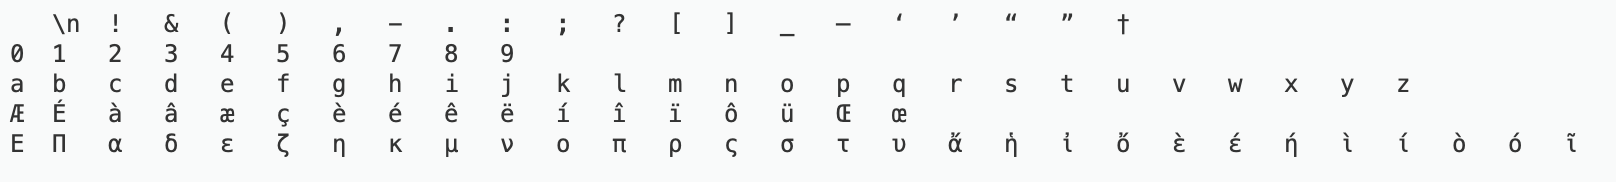
\includegraphics[width=\linewidth]{preprocessed.png}	
		\caption{Unique characters in \textit{The Count of Monte Cristo} after 
		the preprocessing}
		\label{fig:preprocessed}
	\end{figure}
	
	Afterwards, analysing more carefully the frequencies of the characters, it 
	was decided to replace rare characters with the token `\texttt{UNK}'. In 
	particular, all those characters appearing with a frequency less than 
	100 have been considered "rare". In fact, in a text containing 2615988 
	occurrences, 100 are less than $0.004\%$.
	\bigskip
	
	Following, the two dictionaries containing the integer and integer mappings 
	have been recreated.
	\bigskip
	
	\begin{figure}[htb]
		\centering
		\begin{tabular}{llcc}
			\toprule
			Encoding & Characters &  Absolute Frequencies & Relative 
			Frequencies \\
			\midrule
			6        &           &                417112 &              
			15.945\% \\
			5        &         e &                256526 &               
			9.806\% \\
			13       &         t &                178459 &               
			6.822\% \\
			11       &         a &                164051 &               
			6.271\% \\
			1        &         o &                155404 &               
			5.941\% \\
			18       &         i &                140911 &               
			5.387\% \\
			\dots       &         \dots &                \dots 
			&             \dots \\
			52       &       UNK &                   667 &               
			0.025\% \\
			\dots       &         \dots &                \dots 
			&             \dots \\
			\bottomrule
		\end{tabular}
		\captionof{table}{Encoding and frequencies of the characters after the 
			preprocessing}
		\label{tab:statistics2}
	\end{figure}

	In Table \ref{tab:statistics2} are presented the new characters, which this 
	time are only 53, with the corresponding encoding and frequency.
	\bigskip

	The training loss of this experiment is shown in Figure 
	\ref{fig:loss-preprocessed}. At the end of the training, the loss is 
	1.24, so is decreased respect to the experiment without preprocessing.

	\begin{figure}[H]
		\centering
		\includegraphics[width=.7\linewidth]{../src/out/preprocessed/img/loss.pdf}
		\caption{Training loss of the model with preprocessing}
		\label{fig:loss-preprocessed}
	\end{figure}
	\bigskip
	
	\noindent Below are shown some examples of sentences generated after the 
	training of this model:
	
	\begin{shadequote}{}
		madame de villefort\texttt{$\backslash$n}\\
		passed before it glict, the ception of similar smile to the man here, 
		those whisten to\texttt{$\backslash$n}\\
		habituated in their if for him for me, by such about to take pity on 
		chance from the\texttt{$\backslash$n}\\
		young step, to have because entering the assampo, he has the co
	\end{shadequote}

	\begin{shadequote}{}
		’ took so wifterness. he is venecont respectly a 
		labing.”\texttt{$\backslash$n}\\
		\texttt{$\backslash$n}\\
		“and do you are\texttt{$\backslash$n}\\
		already known the first obstatrark seemed her with so partiery were 
		death, only or his bed\texttt{$\backslash$n}\\
		of the grotto\_ gentlemen, ali risk to the 
		days--”\texttt{$\backslash$n}\\
		\texttt{$\backslash$n}\\
		“the\texttt{$\backslash$n}\\
		count,” said monte cristo, as eres
	\end{shadequote}
	
	Also in this experiment, the sentences obtained have poor meaning, but the 
	percentage of existing English words is increase from $80\%$ to $86\%$.
	In this case, much less phrases generated contain multiple new lines.
	Moreover, most of the sentences include proper names such as 
	`\textit{mademoiselle de villefort}' and `\textit{monte cristo}' that comes 
	directly from the book.
	
	\bigskip
	
	One of the easiest thing that is possible to do to improve the results is 
	increasing the number of epochs of the training.
	\bigskip
	
	A new experiment was then carried out: the previous model has been trained 
	for 10 epochs instead of 5. The two trends of the losses are shown the 
	Figures \ref{fig:loss-preprocess-5and10epochs}.
	
	\begin{figure}[htb]
		\begin{minipage}[c]{.485\textwidth}
			\centering
			\includegraphics[width=\linewidth]{../src/out/preprocessed/img/loss.pdf}
			\caption*{(a)}
		\end{minipage}
		~
		\begin{minipage}[c]{.485\textwidth}
			\centering
			\includegraphics[width=\linewidth]{../src/out/preprocessed-10epochs/img/loss.pdf}
			\caption*{(b)}
		\end{minipage}
		\caption{Training loss of the preprocessed models with 5 and 10 epoch 
		training}
		\label{fig:loss-preprocess-5and10epochs}
	\end{figure}
	
	It is clearly visible that the training loss has continued to decrease in 
	the 
	following epochs, reaching 1.12. Table \ref{tab:performace-prepocess} 
	documents the training losses of the first experiment and of the ones with 
	the 
	preprocessing.
	
	\begin{table}[htb]
		\centering
		\begin{tabular}{l@{\hspace{.5cm}}ccc}
			\toprule
			\textbf{Model} & \textbf{Epochs} & \textbf{ training loss} & 
			\textbf{Train Time}  \\
			\midrule
			\texttt{initial}  		&  5 & 1.32 & 768 sec  \\
			\texttt{preprocessing\_5e}  &  5 & 1.24 & 1124 sec \\
			\texttt{preprocessing\_10e}  & 10 & 1.12 & 2267 sec\\
			\bottomrule 
		\end{tabular}
		\captionof{table}{Initial and preprocessed models performances}
		\label{tab:performace-prepocess}
	\end{table}

	\bigskip
	\noindent Below are shown some examples of sentences generated after the 
	training of this model:
	
	\begin{shadequote}{}
		knose eugénie so appreascioully come. my\texttt{$\backslash$n}\\
		mother has entrobited her habyighten light for albert had heard of 
		obligor\texttt{$\backslash$n}\\
		to itiquer some shipowners, or if not that unhappy. besides, let
		me not get. in the ground old man are also, and now it is 
		theref.”\texttt{$\backslash$n}\\
		\texttt{$\backslash$n}\\
		“yet—sa
	\end{shadequote}
	
	\begin{shadequote}{}
		mademoiselle decribidities, has their fortunes at 
		verture\texttt{$\backslash$n}\\
		monsieur, and that he has done by his impassic 
		gegary\texttt{$\backslash$n}\\
		dest on the yacht appeared.”\texttt{$\backslash$n}\\
		\texttt{$\backslash$n}\\
		“you know no other, that there is dead that the plan of myself and the 
		pleasure\texttt{$\backslash$n}\\
		of the different charms, countess
	\end{shadequote}

	Also in this experiment, the sentences obtained are very similar to the 
	previous. 
	Sometimes it can be seen the attempt to generate sentences with a 
	more elaborate grammatical structure. Once again, there are some proper 
	names derived from the book.
	\bigskip
	
	The following experiment proposes the use of a model regularisation 
	technique, that is the addition of a dropout layer after 
	each LSTM cell. In particular, during the training phase, the probability 
	to keep each neuron is set to $0.5$, while during the generation of the 
	sentence is set to $1$.
	\bigskip
	
	The experiment with the dropout has been executed on the initial model and 
	on the one with preprocessing, in both cases for 5 training epochs. Another 
	experiment has been carried out on the experiment with preprocessing for 10 
	training epochs. 

	\bigskip
	In Table \ref{tab:performace-dropout} are summarised the training losses of 
	the  models presented above.
	
	\begin{table}[H]
		\centering
		\begin{tabular}{l@{\hspace{.5cm}}ccc}
			\toprule
			\textbf{Model} & \textbf{Epochs} & \textbf{ training loss} & 
			\textbf{Train Time}  \\
			\midrule
			\texttt{dropout\_5e}  				 &  5 & 1.38 & 1203 sec  \\
			\texttt{dropout+preprocessing\_5e}   &  5 & 1.41 & 1146 sec \\
			\texttt{dropout+preprocessing\_10e}  & 10 & 1.30 & 2268 sec\\
			\bottomrule 
		\end{tabular}
		\captionof{table}{Dropout models performances}
		\label{tab:performace-dropout}
	\end{table}
	
	The new performances are shown in Figure \ref{fig:loss-dropout}. Looking at 
	the loss values, the performances did not improve as expected after the 
	application of the dropout. 
	\begin{figure}[htb]
		\begin{minipage}[c]{.485\textwidth}
			\centering
			\includegraphics[width=\linewidth]{../src/out/dropout/img/loss.pdf}
			\caption*{(a)}
		\end{minipage}
		~
		\begin{minipage}[c]{.485\textwidth}
			\centering
			\includegraphics[width=\linewidth]{../src/out/preprocessed-dropout/img/loss.pdf}
			\caption*{(b)}
		\end{minipage}
		\centering
		\begin{minipage}[c]{.485\textwidth}
			\centering
			\includegraphics[width=\linewidth]{../src/out/preprocessed-dropout-10epochs/img/loss.pdf}
			\caption*{(c)}
		\end{minipage}
		\caption{Training loss of the models with dropout}
		\label{fig:loss-dropout}
	\end{figure}
	\bigskip
	
	\noindent Below are shown some examples of sentences generated after the 
	training of these models. First of all, the \texttt{dropout\_5e} model 
	sentences:
	
	\begin{shadequote}{}
		with a fear of that thing; he counded, and\texttt{$\backslash$n}\\
		that how but ere shall following the hour after himself with him, 
		her\texttt{$\backslash$n}\\
		about like a father in which i have made up wable where they, having 
		not to the\texttt{$\backslash$n}\\
		luminy of little officers, of real, who will a took lice that s
	\end{shadequote}
	
	\begin{shadequote}{}
		ble alone, and kill him and ceunal,\texttt{$\backslash$n}\\
		he silently surprised through a shuspications in\texttt{$\backslash$n}\\
		persons about him demins, they have been signor in a may but his times 
		in ones examined the room elgering. a sordious pessage. one assured 
		escape about done back—they beli
	\end{shadequote}
	
	 \noindent Following the \texttt{dropout+preprocessing\_5e} generated 
	 sentences:
	 \begin{shadequote}{}
	 	ate a king and persons and occupidioned saments to the six months, 
	 	ecchapting by the question. my horsing on the\texttt{$\backslash$n}\\
	 	content\texttt{$\backslash$n}\\
	 	to thrust in if the minister of\texttt{$\backslash$n}\\
	 	done in the peapr was\texttt{$\backslash$n}\\
	 	fortuno would enter all in all the gion, not, and they have dispased to 
	 	her certa
	 \end{shadequote}
	 
	 \begin{shadequote}{}
	 	at this sifficience at\texttt{$\backslash$n}\\
	 	them similary! a present paris, and there he\texttt{$\backslash$n}\\
	 	exactly i have been breathtoms,\texttt{$\backslash$n}\\
	 	as then it am flefts to the brother as the\texttt{$\backslash$n}\\
	 	merening had been about towards the time of two honor, 
	 	now,\texttt{$\backslash$n}\\
	 	peeping, himself, who had piimed albert, shuddered s
	 \end{shadequote}
 
 	\noindent Finally, the \texttt{dropout+preprocessing\_10e} generated 
 	sentences:
	\begin{shadequote}{}
		apped himself announcing laugh. like her more pray. he could not now 
		visit with there the did the judge of series,\texttt{$\backslash$n}\\
		promised into the mother. her sailors shuddered to the idea that he had 
		seemed\texttt{$\backslash$n}\\
		as\texttt{$\backslash$n}\\
		given at murderers. having were ministerings because the ho
	\end{shadequote}
	
	\begin{shadequote}{}
		has dispermined me, you were men he deet of you to filled, you cause 
		that rush to her accommands,—now prayers i can find 
		my\texttt{$\backslash$n}\\
		sound which is\texttt{$\backslash$n}\\
		not since\texttt{$\backslash$n}\\
		all them to mention by dusty police.”\texttt{$\backslash$n}\\
		\texttt{$\backslash$n}\\
		“rean of the correst that was delighted as yourself take preparate,
	\end{shadequote}

	Since the models seem to be underfitting, the following experiment aims is 
	to improve the model's performances by increasing the complexity of the 
	network, in particular, the number of parameters and in general the 
	dimension of the network. To accomplish this, a new LSTM cell is added to 
	the network after the previous, with the same number of hidden-units. 
	\bigskip
	
	The experiment with the additional layer has been executed on the 
	preprocessed model both with and without dropout. Since the results on the 
	model with dropouts are the worst, only those on the model without dropouts 
	will be shown. 
	\bigskip
	
	This experiment has been carried out for both 5 and 10 training epochs.
	\bigskip
	
	In Table \ref{tab:performace-layers} are summarised the training losses of 
	the  models presented above.
	
	\begin{table}[H]
		\centering
		\begin{tabular}{l@{\hspace{.5cm}}ccc}
			\toprule
			\textbf{Model} & \textbf{Epochs} & \textbf{ training loss} & 
			\textbf{Train Time}  \\
			\midrule
			\texttt{preprocessing\_5e}   		 &  5 & 1.24 & 1124 sec \\
			\texttt{preprocessing\_10e}  		 & 10 & 1.12 & 2267 sec\\
			\texttt{preprocessing+3layers\_5e}   &  5 & 1.23 & 1574 sec \\
			\texttt{preprocessing+3layers\_10e}  & 10 & 1.17 & 3113 sec\\
			\bottomrule 
		\end{tabular}
		\captionof{table}{Comparison of the performance of the experiments with 
		preprocessing as the number of layers varies}
		\label{tab:performace-layers}
	\end{table}

	The performances are shown in Figure \ref{fig:loss-layers}.	Looking at the 
	loss values, the performances seem to be very similar to the experiment 
	without the additional layer.
	\begin{figure}[htb]
		\begin{minipage}[c]{.485\textwidth}
			\centering
			\includegraphics[width=\linewidth]{../src/out/preprocessed-3layers/img/loss.pdf}
			\caption*{(a)}
		\end{minipage}
		~
		\begin{minipage}[c]{.485\textwidth}
			\centering
			\includegraphics[width=\linewidth]{../src/out/preprocessed-3layers-10epochs/img/loss.pdf}
			\caption*{(b)}
		\end{minipage}
		\caption{Training loss of the models with an additional layer}
		\label{fig:loss-layers}
	\end{figure}
	

	\bigskip
	
	\noindent Below are shown some examples of sentences generated after the 
	training of these two models. First of all, the 
	\texttt{preprocessing+3layers\_5e} model sentences:
	
	\begin{shadequote}{}
		this man mistrust, i know the valet, is a populurity, and the gilt on 
		it. many, was well he remind him the fair, you are penehed to mention 
		any more, sir, and crossed now nearly.”\texttt{$\backslash$n}\\
		\texttt{$\backslash$n}\\
		“i meanh. the statue, who has a life, come; i\texttt{$\backslash$n}\\
		may, then your recollection.”
	\end{shadequote}
	
	\begin{shadequote}{}
		but what will deceive
		the dream, and villefort did not concernment sitting a man, who in the 
		larger together usuals! what dantès sail at the count 
		it\texttt{$\backslash$n}\\
		was but they princess each straw the understand by the 
		third\texttt{$\backslash$n}\\
		louis where i think of the taking notice? wh
	\end{shadequote}
	
	\noindent Finally, the \texttt{preprocessing+3layers\_10e} generated 
	sentences:
	\begin{shadequote}{}
		don the preuisjest,” exclaimed the count gave you, 
		that\texttt{$\backslash$n}\\
		he heard some years, englest he has impossively for messness of it?” 
		chote me entirelyable successly to auteuil from the island whose 
		theatantly\texttt{$\backslash$n}\\
		pressed much\texttt{$\backslash$n}\\
		anything at such at all the dying places,
	\end{shadequote}
		
	\begin{shadequote}{}
		her son, asred you, you amed france, my mother, enerved with five?” 
		asked d’Épinay, aud valentine,” observed miner.”\texttt{$\backslash$n}\\
		\texttt{$\backslash$n}\\
		dantès would be enough than your father’s affair; it is quarones, and 
		wild you have as bad the phys. and pass of\texttt{$\backslash$n}\\
		the man\texttt{$\backslash$n}\\
		in black careness
	\end{shadequote}

	The sentences generated with this experiment seems to have many more 
	existing English word. The structure of the sentences is improved too. 
	
	\bigskip
	The last experiment performed, used multiple books to train the network. In 
	particular, the books \textit{The Count of Monte Cristo}, \textit{The Three 
	Musketeers} and \textit{The Man In The Iron Mask}, which are all by the 
	same author, namely Alexandre Dumas, have been downloaded in plain English 
	text from Project Gutenberg.
	
	These books contain a total of 4.88 million characters and $104$ unique 
	characters. The character list is displayed in Figure \ref{fig:multibooks}.
	
	\begin{figure}[htb]
		\centering
		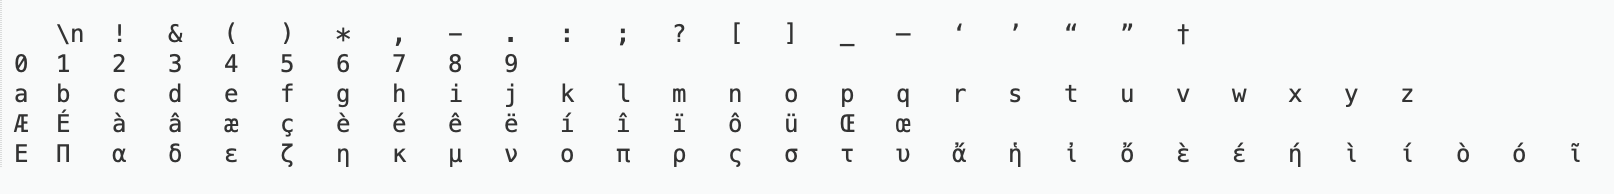
\includegraphics[width=\linewidth]{multibooks.png}	
		\caption{Unique characters in the three books}
		\label{fig:multibooks}
	\end{figure}
	
	After having replaced the rare characters with the token `\texttt{UNK}', 
	the unique characters are $55$. 
	Table \ref{tab:statistics3} presents the characters with the corresponding 
	encoding and frequency.
	
	\begin{figure}[htb]
		\centering
		\begin{tabular}{llcc}
			\toprule
			Encoding & Characters &  Absolute Frequencies & Relative 
			Frequencies \\
			\midrule
			6        &           &                777271 &              
			15.928\% \\
			5        &         e &                475075 &               
			9.736\% \\
			13       &         t &                334958 &               
			6.864\% \\
			11       &         a &                307634 &               
			6.304\% \\
			1        &         o &                288840 &               
			5.919\% \\
			18       &         i &                263412 &               
			5.398\% \\
			\dots       &         \dots &                \dots 
			&             \dots \\
			54       &       UNK &                   556 &               
			0.011\% \\
			\dots       &         \dots &                \dots 
			&             \dots \\
			\bottomrule
		\end{tabular}
		\captionof{table}{Encoding and frequencies of the characters of the 
		three books preprocessed}
		\label{tab:statistics3}
	\end{figure}

	The experiment consists in training the network after applying the previous 
	presented preprocessing procedure.
	The training loss of this experiment is shown in Figure 
	\ref{fig:loss-multibooks}, and the end of the training it is 1.09, the best 
	result reported so far. 
	
	\begin{figure}[H]
		\centering
		\includegraphics[width=.6\linewidth]{../src/out/preprocessed-multibooks/img/loss.pdf}
		\caption{Training loss of the experiment with multiple books}
		\label{fig:loss-multibooks}
	\end{figure}
	\bigskip
	
	\noindent Below are shown some examples of sentences generated by this 
	model:
	
	\begin{shadequote}{}
		one saw so that one morning, really to say, ‘at\texttt{$\backslash$n}\\
		the first heep; it is my mother, dig theolord.”\texttt{$\backslash$n}\\
		\texttt{$\backslash$n}\\
		“harning to me? then, then, who could not appear not to send 
		the\texttt{$\backslash$n}\\
		ill vignitady for him this.”\texttt{$\backslash$n}\\
		\texttt{$\backslash$n}\\
		“and i will not place against your hands and the present 
		is\texttt{$\backslash$n}\\
		goin
	\end{shadequote}
	
	\begin{shadequote}{}
		, suddenly, i will be fated, and have we\texttt{$\backslash$n}\\
		cast and leave barries, but an assistance, and reconsuited 
		myself\texttt{$\backslash$n}\\
		and dressed to hear my arms, and for women. instead of afflinity, 
		whose\texttt{$\backslash$n}\\
		apartments of lines, madame morrel asked any—to wish to obtain the 
		not\texttt{$\backslash$n}\\
		drague
	\end{shadequote}
	

\end{document}
